
%Superscripts and subscripts that are words or abbreviations, as in
%\( \pi_{\mathrm{low}} \), should be typed as roman letters; this is
%done as \verb|\( \pi_{\mathrm{low}} \)| instead of \( \pi_{low} \)
%done by \verb|\( \pi_{low} \)|.

%User-defined macros should be placed in the preamble of the chapter,
%and not at any other place in the document. Definitions made using
%the commands \verb|\newcommand,| \verb|\renewcommand,|
%\verb|\newenvironment| or \verb|\renewenvironment| should be used


\chapter[FFAG]{FFAG}\label{chapFFAG}


\section{Introduction}\label{secFFAGIntro}


\begin{figure}[ht]
\sidebyside
{
  \begin{minipage}{.47\linewidth}
    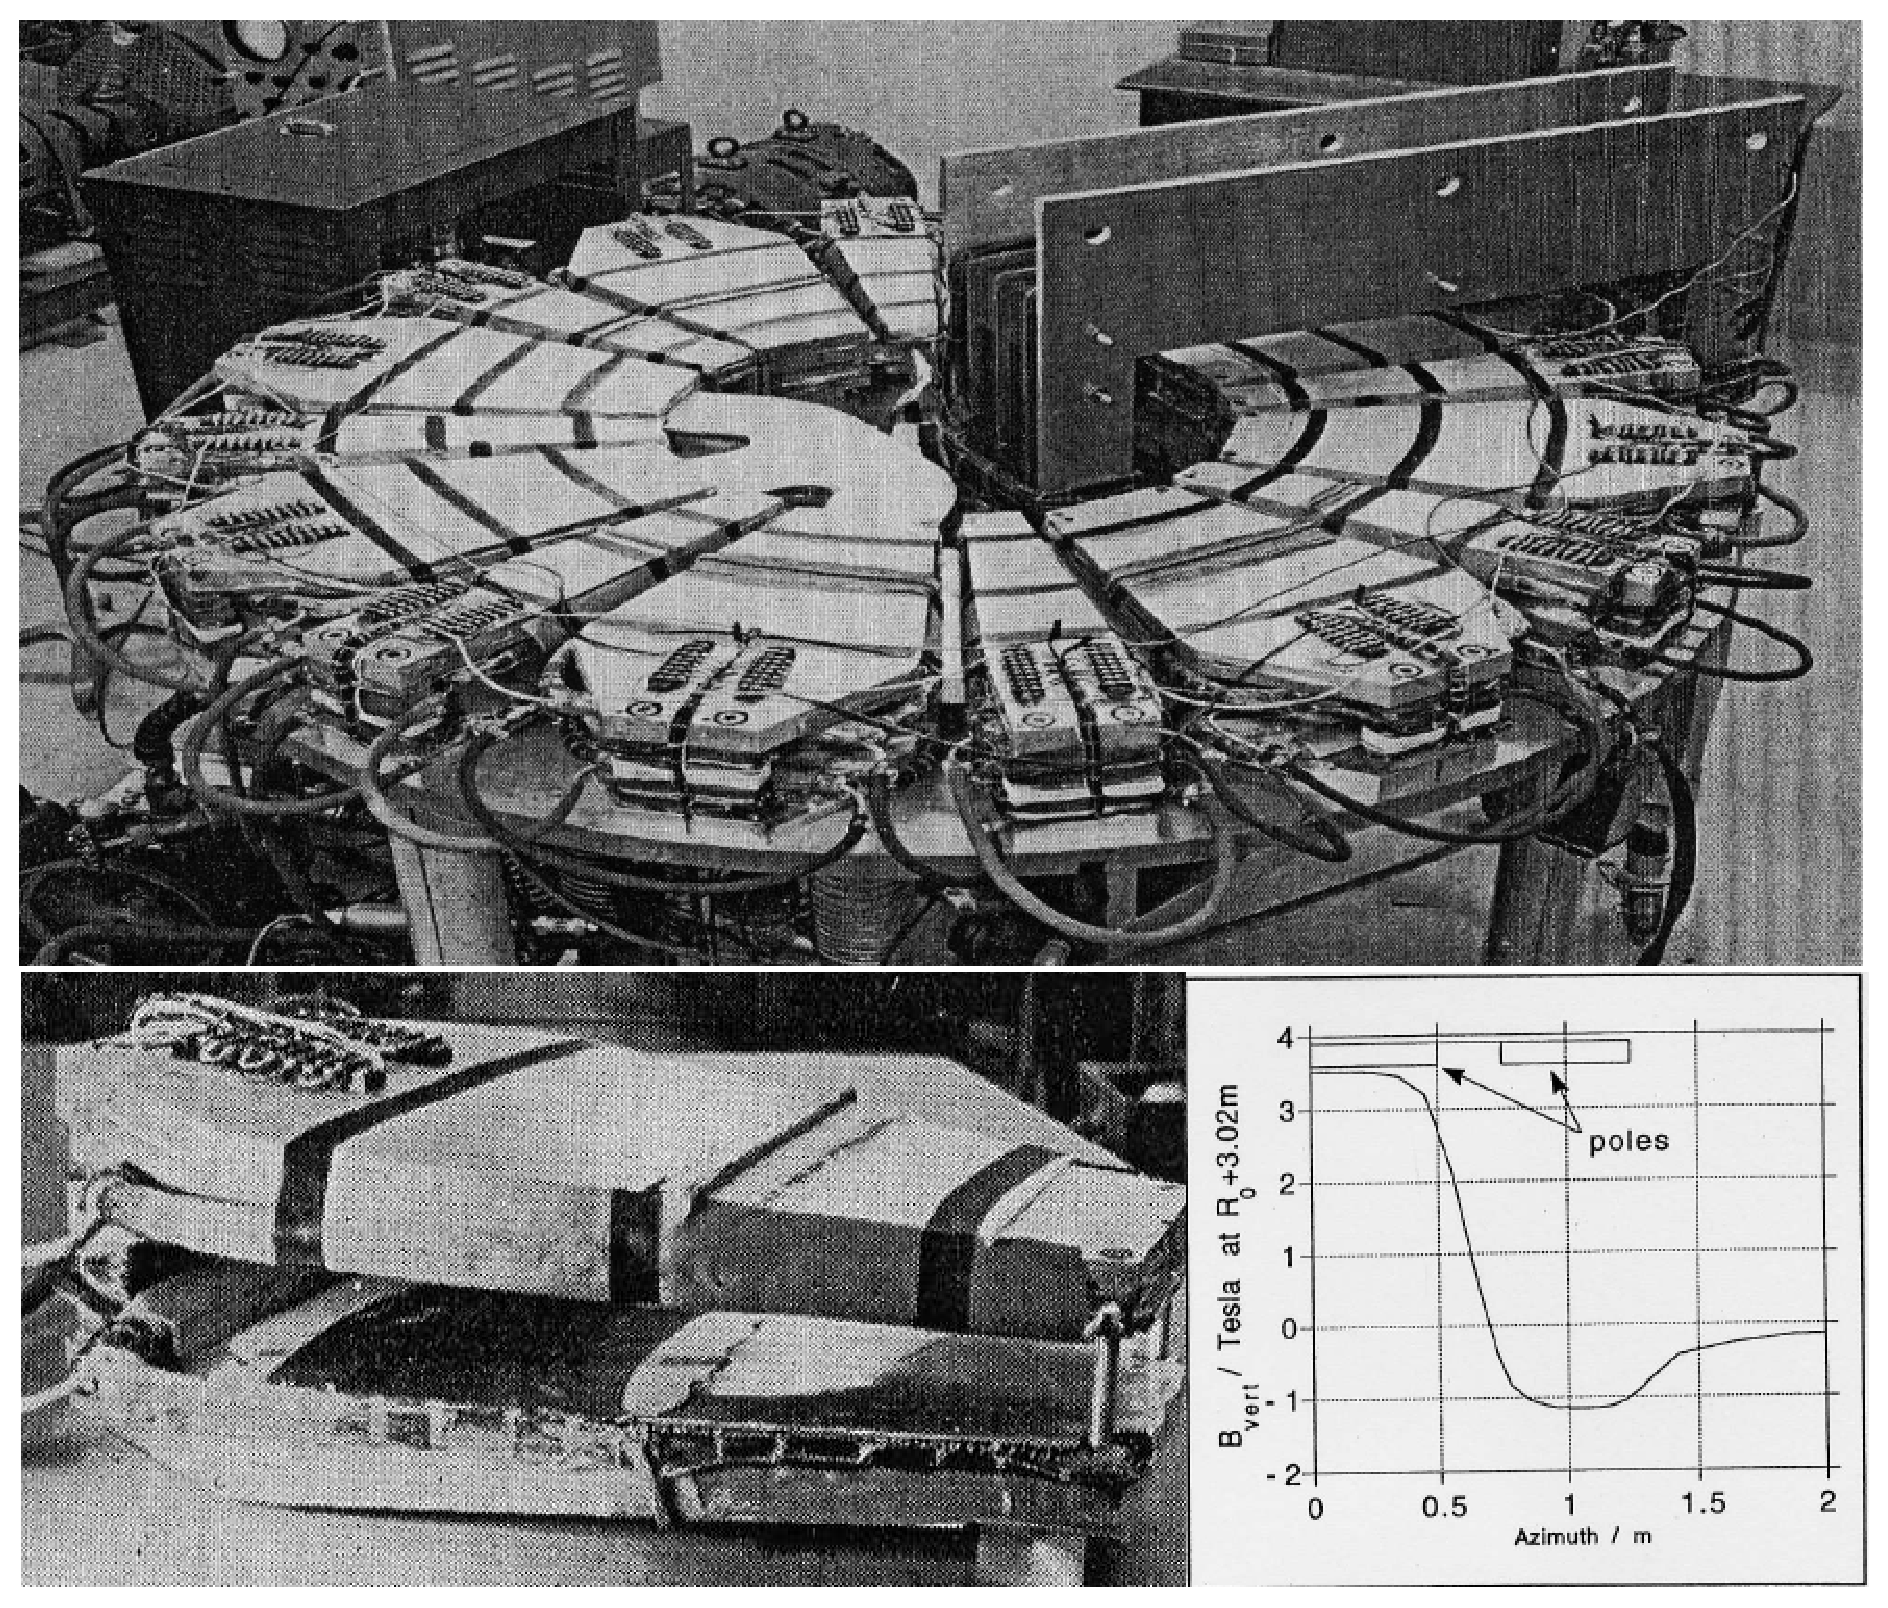
\includegraphics[width=0.99\linewidth]{./figs_ffag/MARKII.eps}
    \caption{
  Top: the DF lattice MURA MARK II and its induciton acceleration system, the 
 first electron FFAG (first beam in 1956 ******)~\cite{BibFFAG-1}.
Bottom: variable gap, defocusing, sector dipole. 
    } 
    \label{figFFAG_MARKII}
   \end{minipage}
}{
  \begin{minipage}{.45\linewidth}
    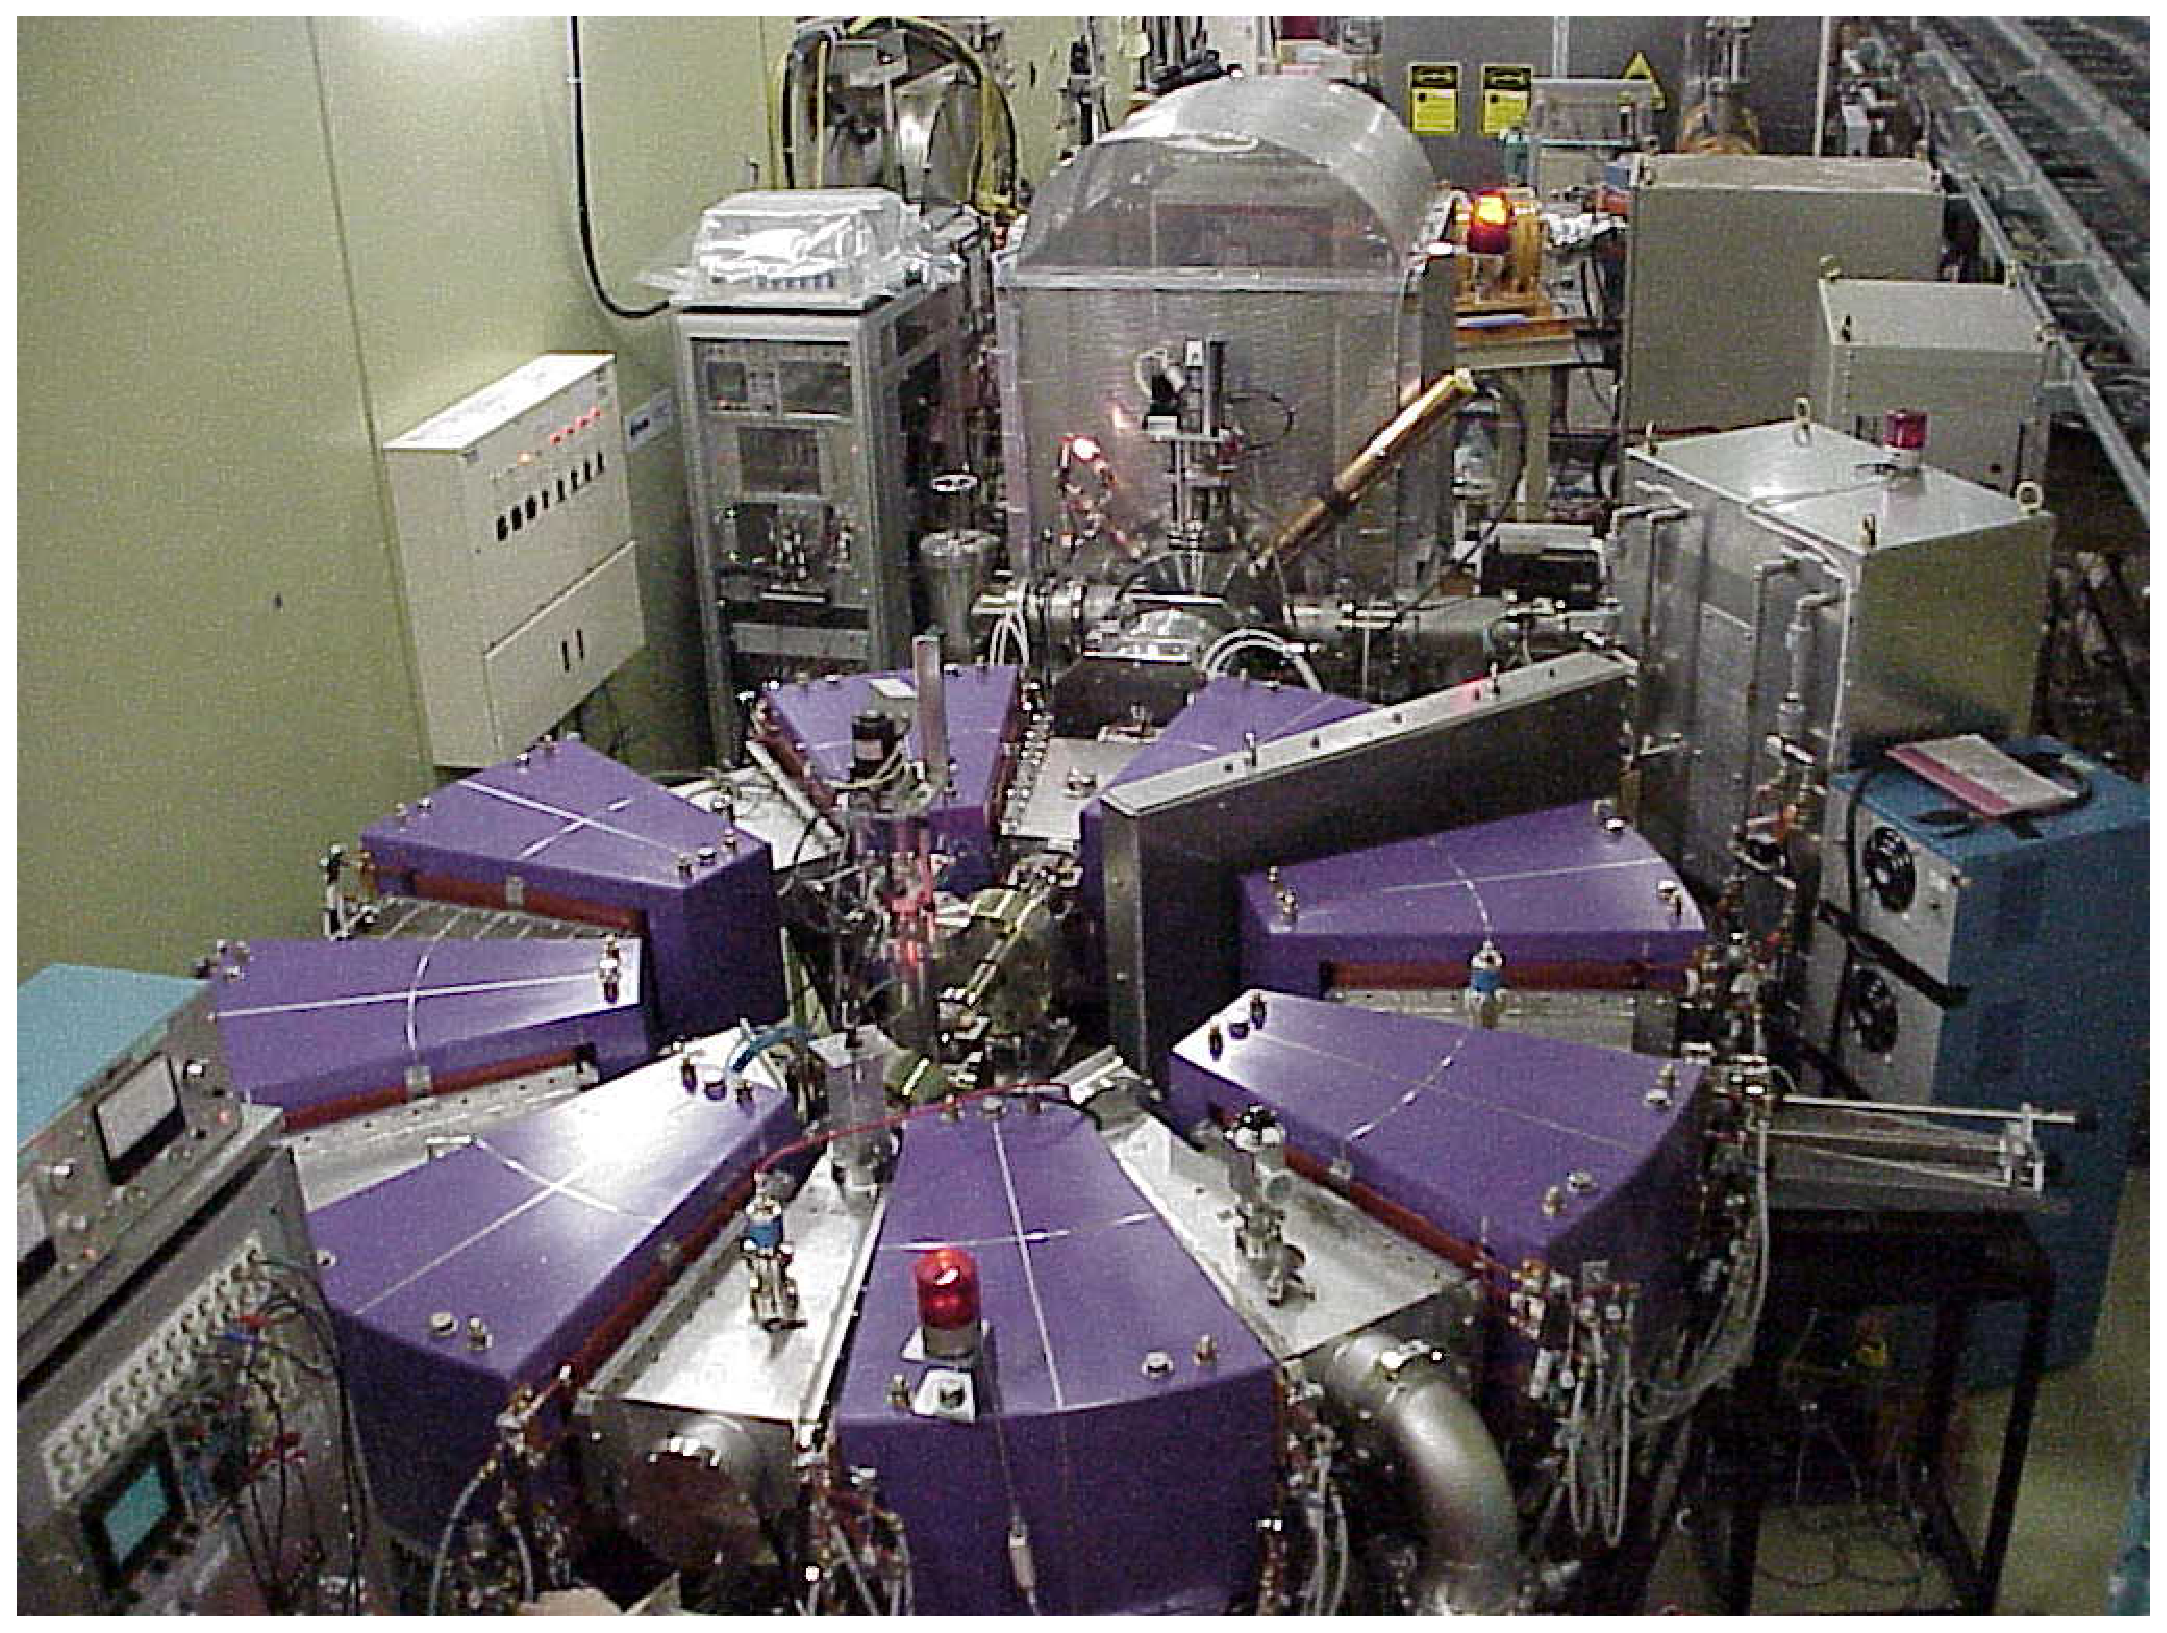
\includegraphics[width=0.99\linewidth,height=2.6cm]{./figs_ffag/PoPFFAG.eps}\\
    \includegraphics[width=0.52\linewidth]{./figs_ffag/popMagnet.eps}
    \includegraphics[width=0.45\linewidth]{./figs_ffag/FFAG31_cavity.eps}
    \caption{
    The first proton FFAG (first beam 1999), particle source 
 in the background, RF system on the right and bottom-right picture, 
DFD triplet sector dipole bottom-left picture~\cite{BibFFAG-2}. 
    }
    \label{figFFAG_POP}
   \end{minipage}
}
\end{figure}

 Fixed Field Alternating Gradient (FFAG) accelerators are separated sector, fixed-field, ring accelerators. 
Fixed field technology allows high repetition rates. 
  Gaps between sectors allow the insertion of dedicated equipmnet for injection, acceleration, extraction, diagnostics, vacuum
(Figs.~\ref{figFFAG_MARKII},~\ref{figFFAG_POP}).
Trajectories in an FFAG lattice spiral under the effect of acceleration (outward in scaling FFAGS, as in cyclotrons, 
possibly inward based on particular lattice properties~\cite{FFAGInWardSpiral}). 

Transverse focussing is based on alternating gradient and Thomas focussing. 
Typical lattice cells include  FD (focussing-defocusing) radial sector doublet (Fig.~\ref{figFFAG_MARKII}), 
 DFD radial  sector triplet (Fig.~\ref{figFFAG_POP}), 
 spiral sector dipole  (Fig.~\ref{figFFAG_RACCAM}), quadrupoel doublet or triplet (Fig.~\ref{figNSFFAGdoublet}).
FFAG optics is strong focussing (large betatron phase advance per cell, 
transverse horizontal and vertical wave numbers have large values) 
 resulting in tight transverse bunch confinement.

FFAGs can operate in two ways: (i)~like synchro-cyclotrons, 
the acceleration is cycled using frequency-modulated 
RF to follow the change in revolution period of the accelerated particles, 
the synchrotron motion ensures longitudinal pahse stability (longitudinal focussing), 
 or (ii)~in a \textsl{quasi-isochronous} mode using fixed frequency accelerating RF, 
for  near-crest acceleration of small phase-extent bunches, no longitudinal phase stability in that case
(Chapter~\ref{chapCyclotron}). 
Both methods result in beam being delivered in bunches, at a repetition rate which, in the former case 
is that of the cycling, in the $10^2\sim 10^3$~Hz range, 
or in the latter case amounts to the accelerating RF frequency (MHz range) or a sub-harmonic. 


\section{Scaling FFAG \label{secSFFAG}}

Scaling FFAG lattice is in general not isochronous (more in Sec.~\ref{SecSFFAGQuasiIsoCrhro}), 
by contrast with cyclotron. This results from a different use of the transverse field index k (Eq.~ref{EqCycloRadialIndex}),
namely, to ensure constant focusing, whereas in cyclotrons it is used to ensure isochronism. 




\subsection{Orbits \label{secSFFAGOrbits}}



\smallskip
\noindent {\small $\bullet$} Exercise~\ref{secSFFAGOrbits}-1 
As part of  this exercise, plots will include theoretical expections from the formulas in the text, 
together with ray-tracing outcomes.
Using the \texttt{FFAG} keyword, 
construct a DFD dipole-triplet cell of a 12-cell ring, with the D and F sectors respectively 10.24 and 3.43~degrees, 
half-drift 4.75~deg, identical D-F and F-D spacings, field index $k=7.6$, 
 injection energy 10~MeV on $R_{\rm inj}=4.5****$~m radius and extraction energy 110~MeV.
In the hard-edge magnet model, 
compute 51~orbits, evenly spaced in kinetic energy, in the  range $R_{\rm inj} <r< R_{\rm ext}$ and
plot $B(r)$ (Eq.~{EqFFAGB}), orbit length $\mathcal{L}(r)$ (Eq.~{EqFFAGOrbitL}), revolution period $T_{\rm rev}(r)$ 
(Eq.~{EqFFAGOrbitT}).
Repeat in a soft-dege magnet model using $C_0-C_5 = $ fringe-field coefficient values in \texttt{FFAG}.

Plot the field along the orbits at 10:110:20~MeV, in the hard-edge and soft-edge models.

Compute the momentum compaction (Eq.~{EqFFAGAlpha}), the transition $\gamma$.


\subsection{Focusing \label{secSFFAGFocus}}

\noindent {\small $\bullet$} Exercise~\ref{secSFFAGOrbits}-2 

Plot the betatron and dispersion functions  at 12, 50 and 100~MeV for cpmparison 
(three separate graphs). 

Plot the radial and axial wave numbers, and the chromaticity, as a function of energy or radius. 

The hard-dege model has no $B_s$ focussing. Please explain why, nevertheless, the model 
does provide first order vertical wedge focusing. 

Why is the vertical tune not constant? What parameter can be used to restore constant vertical tune? 
Fing the corresponding gap shape, appply in the FFAG model and check the new evolution of the vertical 
tune so obtained. 


\subsection{Acceleration}\label{secSFFAGAccel}


The RF gap provides a voltage  
\begin{equation}
\label{EqRCyclo}
V_{\rm RF}(t) =\hat V \cos ........... 
\end{equation}
Particles are accelerated as long as they belong in the $[-90,+90]$~degree phase interval, 
the closer to $\phi=90$~deg, the smaller the number of turns 
(the time interval) necessary to reach the extraction radius of the FFAG.
A deviation of the field B from the isochronous value $2\pi m f_{\rm rev}/q$
will result in a  shift in the arrival phase of the particle at the RF gap amounting to 
\begin{equation}
\label{EqPFPhaseCyclo}
\Delta (\sin \phi) = 2\pi h n \Delta B/B
\end{equation}

 ******* prendre de valeurs R, B, etc. realistes, e.g. in ../biblio/22047216.pdf, 23001796.pdf*******

\smallskip
\noindent {\small $\bullet$} Exercise~\ref{secSFFAGAccel}-1 
Assume an accelerating double-gap  configuration as in Fig.~\ref{figLBLCycloSketch}. 
What is the minimum number of turns  expected  from 5~keV to 10~MeV~? Track a particle over that range, 
play with the RF phase, conclude on the  expectations. 
In a V(t) diagram, plot  the position  of the particle along the V(t) curve at the 
accelerating gap, for a magnetic field defect 
$\Delta B/B= 10^{-4}$, homogeneous, in the previous sector  map. 




\subsection{Focusing  \label{secSFFAGFocus}}

Let $B_r$, $B_y$  be the radial and axial components of the magnetic field, respectively, 
$x=r-R$ a small radial displacement with respect to the reference circular orbit,  
$\omega_{\rm rev} = 2\pi f_{\rm rev} $ the angular frequency of the circular motion. 
The radial and axial  strengths experienced by a particle moving in the vicinity of that reference orbit 
write, to the first order in the radial, $x$,  and axial, $y$, coordinates 
\begin{eqnarray}
\label{EqCycloFoc}
F_x = m \ddot x=  -qvB_y + m\frac{v^2}{r} \approx -q v (B_y|_{x=0} + \frac{\partial B_y}{\partial r}x)  + m\frac{v^2}{R}(1-\frac{x}{R}), & \nonumber \\ 
\textrm{~yielding~}  \ddot x + \omega_r^2 x=0 &  \nonumber \\
F_y= m\ddot y =   qvB_r \approx q v \frac{\partial B_r}{\partial y} y = q v \frac{\partial B_y}{\partial r} y, 
 \textrm{~yielding~}    \ddot{y} - \omega_y^2 y= 0  & ~ ~ ~ 
\end{eqnarray}
wherein 
$\omega_r^2 = \omega_{\rm rev}^2(1+\frac{R}{B}\frac{\partial B_y}{\partial r})$,  
$ \omega_y^2 = \omega_{\rm rev}^2 \frac{R}{B} \frac{\partial B_y}{\partial r}$. 
Focusing by a restoring force appears owing to the use of a magnetic field with radial 
index $k = \frac{R}{B}\frac{\partial B_y}{\partial r}|_{x=0,y=0}$. 
The two quantities 
\begin{equation}
  \nu_r = \omega_r/\omega_{\rm rev} = \sqrt{1+k},   ~ ~ ~ ~ 
 \nu_y=\omega_y /\omega_{\rm rev}  = \sqrt{-k} 
\end{equation}
are known  respectively as the radial and the axial ``wave number'' of 
the oscilatory motion in the neiboring of the reference circular orbit.
Note that $\nu_r^2 + \nu_y^2=1$.
Vertical motion stability requires $k$ to be negative~:  $B_y$ (respectively, the magnet gap) 
is slowly  decreasing (increasing) with radius, restoring force toward the 
median plane. 
Focussing in both radial and axial motions requires $0 < k <-1$, a conditon known as ``weak focusing''.
 Note that  at low energy  the electric field in the 
region of the accelerating gap also contributes to the focusing, an aspect omitted here. 


\smallskip
\noindent {\small $\bullet$} Exercise~\ref{secSFFAGFocus}-1
Plot two particle trajectories that demonstrate the value of the radial wave number in the uniform 
field of Sec.~\ref{secSFFAGClassic}. Conclude on orbit and horizontal motion  stability. 
Derive the  vertical  transport matrix from ray-tracing, conclude on the stability of the vertical motion
in a uniform field.


\smallskip
\noindent {\small $\bullet$} Exercise~\ref{secSFFAGFocus}-2
Back to the field map of exercise~\ref{secSFFAGClassic}-1, or to the analytical model 
of exercise~\ref{secSFFAGClassic}-2: introduce a field index $-1<k<0$. 
Plot the radial and vertical phase space of a 5~MeV ion on a $1\mu$m normalized invariant.  
Compute its radial and axial motion wave numbers, $\nu_r$ and $\nu_y$, 
using two different methods, namely, 1-turn mapping and  Fourrier analysis of multi-turn motion. 
From multiturn tracking, generate the envelope of a 5~MeV beam around the ring FFAG.  


\smallskip
\noindent {\small $\bullet$} Exercise~\ref{secSFFAGFocus}-3
Using either the field map or the analytical model devised in the  exercise~\ref{secSFFAGFocus}-2, 
 plot the energy dependence of the reference orbit radius, $R(E)$. 
Plot  $\nu_r^2 + \nu_y^2$ as a function of radius, compare with the value of the field index. 
On a common graphic, plot the horizontal phase space of the 1, 10, 20, 50~MeV particle motion,
assuming the latter on a $1\mu$m normalized invariant in each case.
Plot the vertical phase space motion for these very energies. 
Plot the components of the field vector experienced by a particle as a function of 
azimutahl angle, over a few turns.


\subsection{Quasi-isochronous scaling FFAG lattice \label{SecSFFAGQuasiIsoCrhro}}

With particular constraints on the field index, 
scaling FFAG lattices can be made \textsl{quasi-isochronous} so allowing the use, as in cyclotrons, of fixed-frequency RF 
for acceleration, with however poor isochronism overcome with brute force RF voltage. 




\section{Non-scaling FFAG \label{secNSFFAG}}



\section{Bibliography}

[BibFFAG-1] MURA, MARKII
O Camelot ??


[BibFFAG-2]
Theme Section: FFAG Accelerators, 
in 
Beam Dynamics Newsletter No. 43, 
Issue Editor C.R. Prior, 
August~2007.



\section{Response to exercises \label{secFFAGExResp}}

\noindent {\small $\bullet$} Exercise~\ref{}-2 

The hard-dege model has no $B_s$ focussing. Nevertheless, the model 
does provide first order vertical wedge focusing due to a kick transform, fortran procedure \textrm{WEDGKI}. 

Why is the vertical tune not constant? Because the gap is assumed constant.

What parameter can be used to restore constant vertical tune? Gap shape $\rm gap \sim 1/r^{\kappa}$, 
with $\kappa\sim$ a few units to be determine. This will cause the firnge field 
extent to have the appropriate $r$-dependence. 
